\documentclass[xcolor=svgnames,dvipsnames,table, hyperref=pdftex, mathserif, presentation]{beamer}
\usepackage{amsmath,amssymb,amsfonts,amsthm}
\usepackage{ctex}
\usepackage{graphics}
\usepackage{graphicx}
\usepackage{xcolor}
\usepackage{wasysym}
\usepackage{bbm}
\usepackage{url}
\usepackage{beamerleanprogress}
\usepackage{tikz-dependency}
\usepackage{tikz-qtree}

\usetheme{CambridgeUS}
%\usetheme{Pittsburgh}
\usecolortheme{orchid} % seahorse  orchid rose
\setbeamertemplate{blocks}[rounded][shadow=true]
\AtBeginSection[]{%
  \begin{frame}<beamer>
    \frametitle{Outline}
      \tableofcontents[current] 
    \end{frame}
  \addtocounter{framenumber}{-1}% If you don't want them to affect the slide number
}
\AtBeginSubsection[]
{
  \begin{frame}
  \frametitle{Outline}
    \tableofcontents[currentsection,currentsubsection]
  %\tableofcontents[sectionstyle=show/hide,subsectionstyle=hide/show/hide]
  \end{frame}
  \addtocounter{framenumber}{-1}% If you don't want them to affect the slide number
}
\newcommand{\setof}[1]{\ensuremath{\left \{ #1 \right \}}}
\newcommand{\tuple}[1]{\ensuremath{\left \langle #1 \right \rangle }}
\newcommand{\red}[1]{\textcolor{red}{#1}}
\newcommand{\brown}[1]{\textcolor{brown}{#1}}
\newcommand{\green}[1]{\textcolor{green}{#1}}
\newcommand{\blue}[1]{\textcolor{blue}{#1}}
\newcommand{\cyan}[1]{\textcolor{cyan}{#1}}

%gets rid of navigation symbols
%\setbeamertemplate{navigation symbols}{}

\begin{document}

\title[中文谓词归一化]{基于中文维基百科构建的\\ 知识库的谓词归一}

\institute[icst.wip@pku]{
  
}
\author[Zhe Han]{\\ 韩喆 \\ iampkuhz@gmail.com
}

\frame[t,plain]{ \titlepage } % [t,plain]

\frame{
  \frametitle{ Outline  }
  
   \begin{itemize}
  \item 背景
    \begin{itemize}
     \item 基于维基百科的知识库
    \end{itemize}
    

  \item Motivation

  \item 实验步骤
  
  \item \textbf{特征选取及分析}.

  \item 实验分析和改进
  \end{itemize}

}

\frame{
  \begin{block}{}
   \begin{center}
    知识库背景
   \end{center}

  \end{block}

}
\frame{
  \frametitle{Background}
  基于中文维基百科(网页)的知识库
	\begin{figure}
	 \begin{minipage}[t]{0.2\linewidth}
	    \centering
	    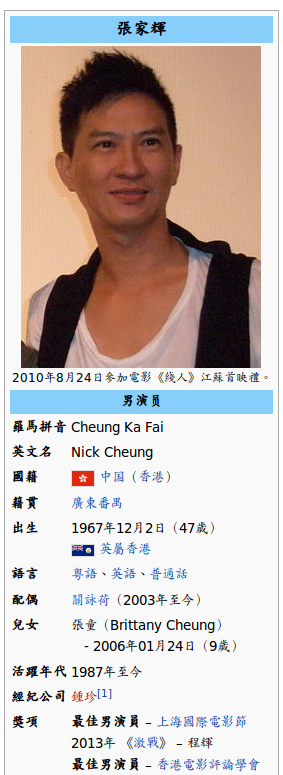
\includegraphics[width=0.8\textwidth]{pic/张家辉.png}
	\end{minipage}
	\begin{minipage}[t]{0.5\linewidth}
	    \centering
	      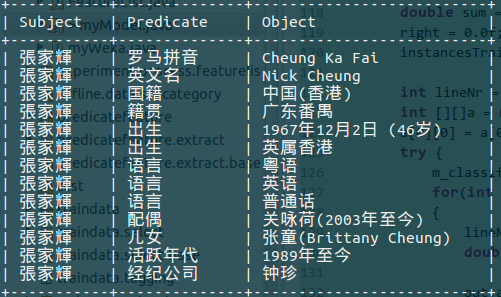
\includegraphics[width=1\linewidth]{pic/张家辉mysql.png}
	\end{minipage}
       \end{figure}
   \begin{itemize}
    \item 330w 三元组, 1.6w个谓词
   \end{itemize}

}


\frame{
  \begin{block}{}
   \begin{center}
    Motivation
   \end{center}

  \end{block}

}

\frame{
    \frametitle{Motivation}
    \begin{enumerate}
     \item 知识库的谓词数量多
	\begin{itemize}
	  \item 1.59w, 手工排查后变成1.4w
	\end{itemize}
    
    \item 谓词冗余
	\begin{block}{含有“邮政”的谓词(17)}
	 INSEE/邮政编码、ISO 3166-2 邮政简写、美国邮政编号、美国邮政编码、邮政、邮政代码、邮政信箱、邮政分区、邮政区号、邮政号码、邮政简称、邮政编号、邮政编号字母、邮政编码、邮政编码FSA、邮政编码首字母、邮政缩写
	\end{block}
    \item 延生查询/知识库合并
	\begin{itemize}
	 \item 推荐相似的谓词给查询者
	 \item 将不同知识库合并时提供谓词归一的规则
	\end{itemize}

    \item \red{所以要进行谓词归一}(没有搜到相关文章)
    \end{enumerate}

}


\frame{
  \begin{block}{}
   \begin{center}
    实验步骤
   \end{center}

  \end{block}

}
\frame{
\frametitle{Method}
    \begin{itemize}
     \item 假设/前提
	\begin{itemize}
	 \item 我们在1.4w个候选谓词内部进行实验
	 \item \textbf{初始问题}:请提供任意两个谓词的相似度,进而判断意义是否相同
	 \item 假设所有字符相同的谓词都是同一谓词,所有字符不同的谓词都非同一谓词
	    \begin{itemize}
	     \item $\times$ \red{姚明}:\blue{出生}:上海 vs \red{刘翔}:\blue{出生地}:上海
	     \item $\surd$ \red{姚明}:\blue{出生}:上海 vs \red{刘翔}:\blue{出生}:1983年7月13日
	    \end{itemize}
	 \item \textbf{转换问题}为二分类:给定任意两个谓词对,判断其是否是相同谓词
	    \begin{itemize}
	     \item 聚类转分类
	     \item 训练数据格式:$[true/false, PredicateId_1, PredicateId_2]$
	     \item 测试数据格式:$[PredicateId_1, PredicateId_2]$
	    \end{itemize}

	\end{itemize}
    \end{itemize}
}

\frame{
  \frametitle{Method}
  \begin{itemize}
   \item 实验环境/数据
	\begin{itemize}
	 \item 自己手工标注了1700多个谓词对
	    \begin{itemize}
	     \item 谓词对本身根据规则(有一定拼音、字符串等相似性)抽取\\ \red{非随机抽取}
	     \item 785个相同谓词对(47.3\%),873个不同谓词对
	    \end{itemize}
	 \item 测试集1000个单词对,训练集500个单词对
	    \begin{itemize}
	     \item 全部分类为true: 52.9\% correct
	    \end{itemize}

	\end{itemize}
  \end{itemize}

}
\frame{
  \frametitle{Method}
  \begin{itemize}
   \item 实验步骤
	\begin{enumerate}
	 \item 对于每个谓词(1/14000),统计其信息(不同类别的特征)
	    \begin{itemize}
	     \item [出生]:pinyin=\{chusheng\},Content=\{出生\},SubjectCategory=\{(篮球运动员,10),(足球运动员,100),(政治人物,50)\}...
	    \end{itemize}

	 \item 对于任意两个谓词,比较其每类特征的相似性,转化为数值,生成特征向量
	    \begin{itemize}
	     \item [出生,出生地]:pinyinSim=0.67, ContentSim=0.67, SubjectCategorySim=0.38,...
	    \end{itemize}
	 \item 对于训练数据,提取特征向量,训练模型
	 \item 对于测试数据,提取特征向量,根据模型预测是否为同一谓词
	\end{enumerate}
  \end{itemize}

}


\frame{
  \begin{block}{}
   \begin{center}
    特征选取及分析
   \end{center}

  \end{block}

}

\frame{
  \frametitle{Method}
  \begin{itemize}
   \item 已选特征
      \begin{itemize}
       \item 文本相似度
       \item 拼音相似度
       \item 词频相似度
       \item wikitext相似度
       \item 主体的类别相似度
      \end{itemize}

  \end{itemize}

}

\frame{
  \frametitle{Method}
  \begin{itemize}
   \item 文本相似度
      \begin{enumerate}
       \item 相同单词个数/总长度 (2维)
       \item $min($编辑距离/总长度$,1)$ (2维)
       \item 61.8\% correct on SVM
      \end{enumerate}
      
   \item 拼音相似度
      \begin{enumerate}
       \item 同文本相似度计算方式,比较字符相同时改用拼音判段是否相同
       \item 53.3\% correct on SVM
      \end{enumerate}
      
   \item 词频相似度
      \begin{enumerate}
       \item 初衷是希望出现频率差别越大的谓词越应当合并(判重),实际基本没有效果
      \end{enumerate}
   
  \end{itemize}

}

\frame{
  \frametitle{Method}
  \begin{itemize}
   \item \red{wikitext相似度}:期望的重点
	\begin{figure}
	 \begin{minipage}[t]{0.45\linewidth}
	    \centering
	    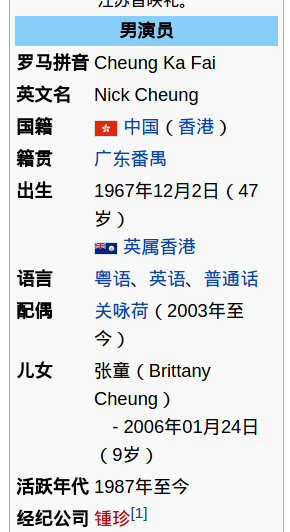
\includegraphics[width=0.6\textwidth]{pic/张家辉info.png}
	\end{minipage}
	\begin{minipage}[t]{0.45\linewidth}
	    \centering
	      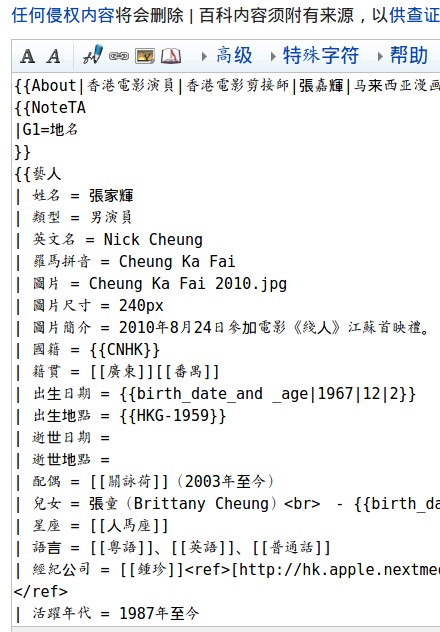
\includegraphics[width=0.8\linewidth]{pic/张家辉wikitext.png}
	\end{minipage}
       \end{figure}
      \begin{itemize}
       \item 出生<=>出生日期,儿女<=>兒女...
      \end{itemize}

  \end{itemize}

}

\frame{
  \frametitle{Method}
  \begin{itemize}
   \item \red{wikitext相似度}.
      \begin{itemize}
       \item 没有固定的对应规则
	  \begin{itemize}
	   \item (比方说)编辑者在“Template:男艺人”页面写了一个转换说明,把“出生日期”自动转化为“出生”显示。如果没有定义,则用模板“Template:人物”的规则匹配。且说明页面非结构化,不能自动抽
	  \end{itemize}

       \item 收集了从wikitext抽取的三元组,利用手写规则与从网页抽取的三元组做对应,然后做统计
       
       \pause
       
	  \begin{block}{内核类别}
	      \begin{itemize}
	       \item \{(kernel type,132),(screenshot,2),(logo,2),(name,2),(kernel,1) \}
	      \end{itemize}
	  \end{block}


	  \begin{block}{出生}
	      \begin{itemize}
	       \item \{(birth place,11470),(birth date,7598),(出生地点,7241),(出生日期,6789),(date of birth,3775),(place of birth,3690),(term start,2346),(出生地,2076),(term end,1511),(birthplace,1156)...\}
	      \end{itemize}

	      
	  \end{block}

	  


      \end{itemize}

   
  \end{itemize}

}

\frame{
  \frametitle{Method}
  \begin{itemize}
    \item \red{wikitext相似度}.
	\begin{itemize}
	  \item 实验效果
		\pause
	    \begin{itemize}
	      \item SVM分类失败(全部预测为1...)
	    \end{itemize}
		\pause
	 \item 失败原因
	    \begin{itemize}
	     \item 80\%的测试数据的相似值为0。很多时候有一个谓词没有对应的wikitext,尤其是出现频率少的谓词
	    \end{itemize}

	 \item 下一步修正
	    \begin{itemize}
	     \item 观察没有抽到wikitext的谓词信息,修改代码(理论上都是可以对应有wikitext的)
	    \end{itemize}

	\end{itemize}
	  
  \end{itemize}

}

\frame{
  \frametitle{Method}
  \begin{itemize}
   \item 主体的类别相似度 \textbf{二级类别分布}。
      \begin{itemize}
       \item 假设前提:\textbf{意义相同的谓词,其所在的三元组的主体的类型分布应该是一致的}.
	  \begin{itemize}
	   \item “\blue{出生}”的主语类别分布\{(人物,10000),(动物,100)\}\\ “\blue{出生日期}”的主语类别分布\{(人物,2000),(动物,500)\}
	  \end{itemize}

       \item 实验方法
	  \begin{itemize}
	   \item 利用中文维基百科的类别,“页面分类”下面的子类(22-2)作为类别分布的规约终点
	      \begin{block}{}
	       语言, 跨學科領域, 应用科学, 文学, 艺术, 宗教, 休閒, 科技, 心理学, 人物, 地理, 人文學科, 技术, 社会, 历史, \red{幫助}, 資訊, 科学, \red{總類}, 自然科学, 社会科学, 哲学, 
	      \end{block}

	      
	   
	   \end{itemize}

      \end{itemize}

  \end{itemize}

}

\frame{
  \frametitle{Method}
  \begin{itemize}
   \item 主体的类别相似度 \textbf{二级类别分布}。
      \begin{itemize}
	   \item 利用维基百科的类别体系,建立所有类别到这22个类别的对应关系
  \begin{figure}[h]
  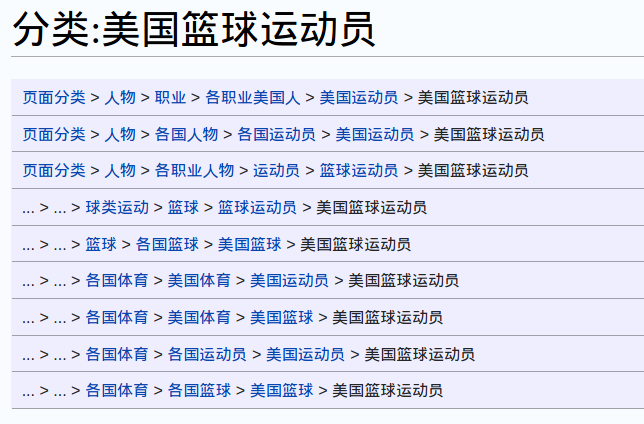
\includegraphics[width=0.5\textwidth]{pic/categoryHirarchy.png}
  \end{figure}
	    \item 20个节点\textbf{宽度优先}向下搜索
		\begin{itemize}
		 \item 深度优先失败,所有类别都是\blue{语言}的子类
		\end{itemize}
		
	    \item “\red{雷·阿伦}:\blue{出生}:加利福尼亚州”\\ \red{雷·阿伦}属于类别“美国篮球运动员”\\ \blue{出生}:\{(人物,100),(科技,10),...\} -> \{(人物,101),(科技,10),...\}
	  
      \end{itemize}

  \end{itemize}

}


\frame{
  \begin{block}{}
   \begin{center}
    总结
   \end{center}

  \end{block}

}

\frame{
  \frametitle{Method}
  \begin{itemize}
   \item 目前效果
      \begin{itemize}
       \item 69.1\% correct on SVM; f1: 0.713
	  \begin{itemize}
	   \item 类别信息、wikitext特征虽然有,但是bug太多\\ 觉得应该做到80\%左右是可以接受的程度
	  \end{itemize}
       \item 二级类别分布特征还在(bu)改(ren)进(zhi)中(shi)...
      \end{itemize}
   
       \item 当时抽特征的时候,没有及时仔细检查,能跑出结果就行...
  \end{itemize}
}


\frame{
  \begin{block}{}
   \begin{center}
    实验分析和改进
   \end{center}

  \end{block}

}
\frame{
  \frametitle{Method (to do)}
  \begin{itemize}
   \item 下一步工作
      \begin{enumerate}
       \item 类别信息特征bug
       \item 规约类别修正
	  \begin{itemize}
	   \item \green{科学}是\green{自然科学}的父类,但都是规约重点
	   \item 类别分布向量直接加入特征向量\\ 原来是做的余弦相似度的值
	  \end{itemize}
       
       \item 增加含有wikitext信息的谓词数量
       \item 频率特征重利用
	  \begin{itemize}
	   \item \red{待完善思路}:频率低的谓词,应当抽取其客体的语义信息
	  \end{itemize}

       \item 命名实体类别分布特征
	  \begin{itemize}
	   \item freebase.NER 提供了维基百科实体的映射关系\\ 通过type->People的类别判断freebase实体的类型\{people,Location,organization,other\}
	  \end{itemize}

      \end{enumerate}

  \end{itemize}
}

\frame{
  \begin{center}
   any uestions || any suggestions ?
  \end{center}

}
\end{document}
